\documentclass[12pt,letterpaper]{article}
\usepackage{graphicx,textcomp}
\usepackage{natbib}
\usepackage{setspace}
\usepackage{float}
\usepackage{fullpage}
\usepackage{color}
\usepackage[reqno]{amsmath}
\usepackage{amsthm}
\usepackage{fancyvrb}
\usepackage{amssymb,enumerate}
\usepackage[all]{xy}
\usepackage{endnotes}
\usepackage{lscape}
\newtheorem{com}{Comment}
\usepackage{float}
\usepackage{hyperref}
\newtheorem{lem} {Lemma}
\newtheorem{prop}{Proposition}
\newtheorem{thm}{Theorem}
\newtheorem{defn}{Definition}
\newtheorem{cor}{Corollary}
\newtheorem{obs}{Observation}
\usepackage[compact]{titlesec}
\usepackage{dcolumn}
\usepackage{tikz}
\usetikzlibrary{arrows}
\usepackage{multirow}
\usepackage{xcolor}
\newcolumntype{.}{D{.}{.}{-1}}
\newcolumntype{d}[1]{D{.}{.}{#1}}
\definecolor{light-gray}{gray}{0.65}
\usepackage{url}
\usepackage{listings}
\usepackage{color}

\definecolor{codegreen}{rgb}{0,0.6,0}
\definecolor{codegray}{rgb}{0.5,0.5,0.5}
\definecolor{codepurple}{rgb}{0.58,0,0.82}
\definecolor{backcolour}{rgb}{0.95,0.95,0.92}

\lstdefinestyle{mystyle}{
	backgroundcolor=\color{backcolour},   
	commentstyle=\color{codegreen},
	keywordstyle=\color{magenta},
	numberstyle=\tiny\color{codegray},
	stringstyle=\color{codepurple},
	basicstyle=\footnotesize,
	breakatwhitespace=false,         
	breaklines=true,                 
	captionpos=b,                    
	keepspaces=true,                 
	numbers=left,                    
	numbersep=5pt,                  
	showspaces=false,                
	showstringspaces=false,
	showtabs=false,                  
	tabsize=2
}
\lstset{style=mystyle}
\newcommand{\Sref}[1]{Section~\ref{#1}}
\newtheorem{hyp}{Hypothesis}

\title{Problem Set 2}
\date{Due: October 22, 2026}
\author{Applied Stats/Quant Methods 1}

\begin{document}
	\maketitle
	\section*{Instructions}
\begin{itemize}
	\item Please show your work! You may lose points by simply writing in the answer. If the problem requires you to execute commands in \texttt{R}, please include the code you used to get your answers. Please also include the \texttt{.R} file that contains your code. If you are not sure if work needs to be shown for a particular problem, please ask.
	\item Your homework should be submitted electronically on GitHub.
	\item This problem set is due before 23:59 on Thursday October 22, 2026. No late assignments will be accepted.

\end{itemize}

	
	\vspace{.5cm}
	\section*{Question 1: Political Science}
		\vspace{.25cm}
	The following table was created using the data from a study run in a major Latin American city.\footnote{Fried, Lagunes, and Venkataramani (2010). ``Corruption and Inequality at the Crossroad: A Multimethod Study of Bribery and Discrimination in Latin America. \textit{Latin American Research Review}. 45 (1): 76-97.} As part of the experimental treatment in the study, one employee of the research team was chosen to make illegal left turns across traffic to draw the attention of the police officers on shift. Two employee drivers were upper class, two were lower class drivers, and the identity of the driver was randomly assigned per encounter. The researchers were interested in whether officers were more or less likely to solicit a bribe from drivers depending on their class (officers use phrases like, ``We can solve this the easy way'' to draw a bribe). The table below shows the resulting data.

\newpage
\begin{table}[h!]
	\centering
	\begin{tabular}{l | c c c }
		& Not Stopped & Bribe requested & Stopped/given warning \\
		\\[-1.8ex] 
		\hline \\[-1.8ex]
		Upper class & 14 & 6 & 7 \\
		Lower class & 7 & 7 & 1 \\
		\hline
	\end{tabular}
\end{table}

\begin{enumerate}
	
\item [(a)] Calculate the $\chi^2$ test statistic by hand/manually (even better if you can do "by hand" in \texttt{R}).\\
{\large \textbf{Assumptions of the chi-square test of independence}}

\begin{enumerate}
	\item \textbf{Categorical variables:} Both variables must be categorical.
	\begin{itemize}
		\item Driver class: upper class or lower class.
		\item Police outcome: not stopped, bribe requested, or stopped/given warning.
	\end{itemize}
	
	\item \textbf{Independence of observations:} Each encounter must be independent of the others.
	
	\item \textbf{Expected cell frequencies:} The expected frequency in each cell should generally be at least 5 for the chi-square approximation to be reliable.
	
	\item \textbf{Random sampling or assignment:} Observations should ideally be randomly sampled. In this study, driver identity was randomly assigned per encounter, but this does not guarantee that all encounters are independent.
\end{enumerate}

{\large \textbf{Hypotheses}}

\begin{enumerate}
	\item $H_0$: The variables are statistically independent.
	\item $H_1$: The variables are statistically dependent.
\end{enumerate}

\lstinputlisting[
language=R,
firstline=34,
lastline=59
]{C:/Users/chane/Desktop/StatsI_2026/problem_sets/PS02/my_answers/PS02_answersCVH.R}

{\large \textbf{Conclusion}}
The calculated chi-square test statistic is $\chi^2 = 3.7912$,
with 2 degrees of freedom and a p-value of approximately $0.1502$.
Since the p-value is greater than the significance level of $0.05$
(5\%), we fail to reject the null hypothesis ($H_0$).
Therefore, there is insufficient statistical evidence to conclude
that social class and police outcome are associated.

Although a warning was issued due to the small sample size and low
expected cell frequencies, the result is not statistically
significant at the 5\% level. However, we cannot conclude that
the variables are independent; we can only say that the data do
not provide sufficient evidence of an association.
\vspace{1cm}
\item [(b)] Calculate the p-value from the test statistic you just created (in \texttt{R}).
\footnote{Remember frequency should be $> 5$ for all cells, but let's calculate the p-value here anyway.}
What do you conclude if $\alpha = 0.1$?

The p-value is approximately $0.1502$.
Since the p-value is greater than the significance level of $0.1$
(10\%), we fail to reject the null hypothesis ($H_0$). Therefore, we fail to reject the null hypothesis as there is insufficient statistical evidence at the (10\%) significance level to conclude that social class and the outcome category are associated.

	
	\newpage
	\item [(c)] Calculate the standardized residuals for each cell and put them in the table below.
	\vspace{1cm}
	
\begin{table}[h]
	\centering
	\begin{tabular}{l | c c c}
		& Not Stopped & Bribe requested & Stopped/given warning \\
		\hline
		Upper class & 0.3220 & -1.6419 & 1.5230 \\
		Lower class & -0.3220 & 1.6420 & -1.5230 \\
		\hline
	\end{tabular}
\end{table}
	\lstinputlisting[
	language=R,
	firstline=82,
	lastline=88
	]{C:/Users/chane/Desktop/StatsI_2026/problem_sets/PS02/my_answers/PS02_answersCVH.R}
	

\vspace{1cm}
\item[(d)] How might the standardized residuals help you interpret the results?

% Include the relevant R code
\lstinputlisting[
language=R,
firstline=95,
lastline=130
]{C:/Users/chane/Desktop/StatsI_2026/problem_sets/PS02/my_answers/PS02_answersCVH.R}

\vspace{0.11cm}
While none of the individual cell residuals exceed the strict standard threshold of $\pm 1.96$ for statistical significance, the data suggests a clear pattern: Lower-class drivers experience a higher rate of bribe requests if they were stopped, whereas upper-class drivers are more likely to receive standard warnings or legitimate stops.
\begin{figure}[htbp]
	\centering
	\includegraphics[width=0.8\textwidth]
	{C:/Users/chane/Desktop/StatsI_2026/problem_sets/PS02/my_answers/Figures/SR_adjusted_scatterplot.png}
	\caption{Scatterplot of Adjusted Standardized Residuals}
	\label{fig:SR_adjusted}
\end{figure}


\end{enumerate}
\newpage


\section*{Question 2: Economics}
Chattopadhyay and Duflo were interested in whether women promote different policies than men.\footnote{Chattopadhyay and Duflo. (2004). ``Women as Policy Makers: Evidence from a Randomized Policy Experiment in India. \textit{Econometrica}. 72 (5), 1409-1443.} Answering this question with observational data is pretty difficult due to potential confounding problems (e.g. the districts that choose female politicians are likely to systematically differ in other aspects too). Hence, they exploit a randomized policy experiment in India, where since the mid-1990s, $\frac{1}{3}$ of village council heads have been randomly reserved for women. A subset of the data from West Bengal can be found at the following link: \url{https://raw.githubusercontent.com/kosukeimai/qss/master/PREDICTION/women.csv}\\

\noindent Each observation in the data set represents a village and there are two villages associated with one GP (i.e. a level of government is called "GP"). Figure~\ref{fig:women_desc} below shows the names and descriptions of the variables in the dataset. The authors hypothesize that female politicians are more likely to support policies female voters want. Researchers found that more women complain about the quality of drinking water than men. You need to estimate the effect of the reservation policy on the number of new or repaired drinking water facilities in the villages.
\vspace{0.1cm}

\begin{figure}[H]
	\centering
	\caption{\footnotesize Names and description of variables from Chattopadhyay and Duflo (2004).}
	\label{fig:women_desc}
	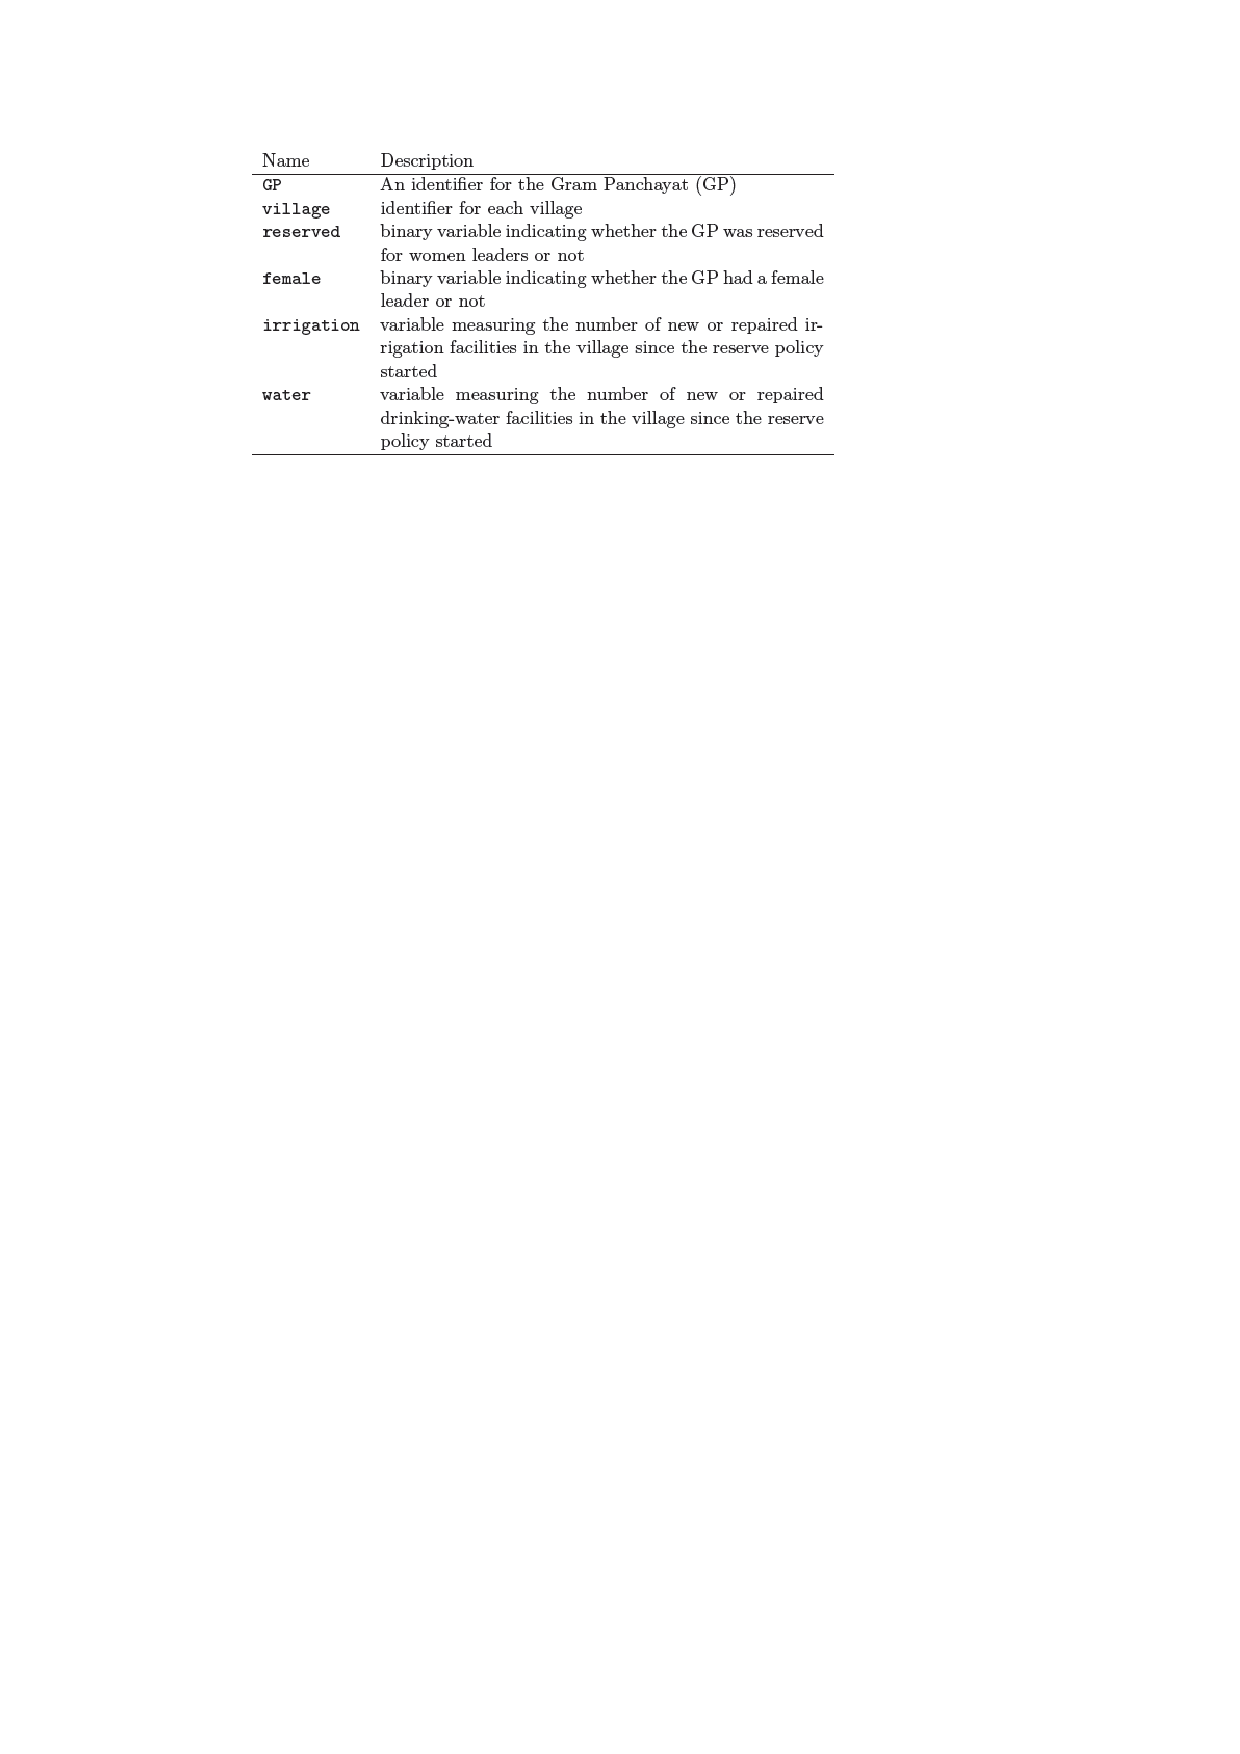
\includegraphics[
	width=1.0\textwidth,
	height=1.0\textheight,
	keepaspectratio
	]{Figures/women_desc.pdf}
\end{figure}

\newpage
\begin{enumerate}
	\item [(a)] State a null and alternative (two-tailed) hypothesis. 
	
	{\large \textbf{Assumptions}}
	
	We assume that the reservation policy was randomly assigned, making the treatment and control groups comparable on average. The analysis also assumes that observations are independent and that the status of one village does not influence the status of another. However, outcomes may be correlated within councils. Since two villages are associated with each Gram Panchayat (GP), this clustering may affect the standard errors. Random assignment helps identify the causal effect, but it does not guarantee independent observations or eliminate all potential issues with statistical inference.
	
	The unit of random assignment is the GP, rather than the individual village. The dataset contains 322 village-level observations corresponding to approximately 161 GPs, with two villages per GP. The treatment group consists of villages in GPs reserved for female leaders (\texttt{reserved = 1}), while the control group consists of villages in GPs not reserved for female leaders (\texttt{reserved = 0}).
	
	\vspace{0.3cm}
	
	{\large \textbf{Hypotheses}}
	
	The null hypothesis states that the reservation policy has no effect on the average number of drinking-water facilities, whereas the alternative hypothesis states that the policy has an effect, either increasing or decreasing the average number of facilities. Formally, the hypotheses are:
	
	\[
	H_0: \beta_1 = 0
	\]
	
	\[
	H_1: \beta_1 \neq 0
	\]
	
	Here, $\beta_1$ represents the population regression coefficient associated with the reservation policy.
	
	\begin{table}[htbp]
		\centering
		\caption{Description of Variables}
		\label{tab:variables}
		\begin{tabular}{l | p{9cm}}
			\hline
			\textbf{Variable} & \textbf{Data Type} \\
			\hline
			GP & Categorical identifier for the GP \\
			village & Categorical identifier for the village within a GP \\
			reserved & Binary (0 = not reserved, 1 = reserved) \\
			female & Binary (0 = male leader, 1 = female leader) \\
			irrigation & Quantitative, discrete count \\
			water & Quantitative, discrete count (outcome variable) \\
			\hline
		\end{tabular}
	\end{table}
	\vspace{6cm}
	\item [(b)] Run a bivariate regression to test this hypothesis in \texttt{R} (include your code!).
	\lstinputlisting[
	language=R,
	firstline=239,
	lastline=243
	]{C:/Users/chane/Desktop/StatsI_2026/problem_sets/PS02/my_answers/PS02_answersCVH.R}
	
The regression results show that the coefficient for female reservation is 
9.252, with a standard error of 3.948 and a \(t\)-statistic of 2.344. 
The \(p\)-value is 0.0197, which is below the 5\% significance level. 
Therefore, we reject the null hypothesis that the coefficient is zero.
	\vspace{0.1cm}
	
The 95\% confidence interval for the estimated coefficient is approximately 
\([1.48, 17.02]\). The \(R^2\) value is 0.0169, meaning that the model 
explains approximately 1.69\% of the variation in the number of 
drinking-water facilities across villages. Since two villages belong to each Gram Panchayat (GP), standard errors 
should ideally be clustered at the GP level.
	\vspace{1cm}
	\item [(c)] Interpret the coefficient estimate for reservation policy. 
	
	The coefficient estimate for the reservation policy is 9.252. This means that villages in Gram Panchayats (GPs) reserved for female leaders had, on average, approximately 9.25 more new or repaired drinking-water facilities than villages in non-reserved GPs.
	
	The intercept of 14.738 indicates that non-reserved GPs had an average of approximately 14 facilities. The estimated average for reserved GPs was therefore 24 facilities for villages in GPs reserved for female leaders.
	\[
	\widehat{\text{water}} = 14.738 + 9.252(\text{reserved})
	\]
		\vspace{0.5cm}
	
	Overall, the positive coefficient suggests that female-leadership reservation is associated with an increase in drinking-water facilities. However, this bivariate regression does not control for other factors that may influence the number of facilities, so the result should not automatically be interpreted as causal.
\end{enumerate}


%\end{enumerate}
\end{document}
